\chapter{Fundamentals of Optics}
\label{chap:theory1}
%- Hva karakterieserer plast utifra hva vi vet
%- ulike sensorer for deteksjon og kartlegging (vise sammenhengen til dette og en bredere oversikt - dette blir isåfall bare her, men tas ikke med videre - i metode kan vi heller si at vi avgrenser mot cam)
%- aktuelle sensorer 
%- sensorbærende plattform
%- PCA og singular value Decomp

In order to understand how an image is retrieved at the end of a spectrometer, knowledge regarding properties of light, is important. This chapter therefore describes the fundamentals of light, its behavior and how it can be utilized. Light has different properties in different environments, determining the degree of utilization. The lecture notes from TTK20 \todo{[kilde]} have been used in large part throughout this chapter. The following sections have this reference as their main reference: \ref{sec:light} Light, \ref{sec:interference} Interference, \ref{sec:diffraction} Diffraction, \ref{sec:grism} The GRISM, \ref{sec:photons} Properties of Photons and \ref{sec:sysopt} System Optics. 

\section{Light} \label{sec:light}
%Color Registration of Underwater Images for Underwater Sensing with Consideration of Light Attenuation
%https://ieeexplore.ieee.org/stamp/stamp.jsp?tp=&arnumber=4209801
Light is electromagnetic radiation. The human eye can detect electromagnetic radiation within wavelengths of 400 and 750 nm, approximately. This electromagnetic spectrum is called visible light. Radiation with shorter wavelength than 400 nm is called ultraviolet, whereas infrared radiation has longer wavelength than visible light.
\\\\
When light from a light source hits an object surface, the light is reflected before eventually reaching the eye. In this task, the endpoint will not only be the human eye, but other viewpoints, for instance a camera lens. The observation of the reflected colors in the viewpoint, is affected by properties of object surfaces, the light intensity of light source and traveling distance of the light.
\\\\
%PDF FRA TTK20
Breaking down the definition of light, light can be defined as tiny packets called photons. The properties addressed to the photons are wave like. Because of this, the wave of light can be represented as a sine wave. The wave amplitude in 2D can be expressed as follows: 

\begin{equation}
    E(x,t) = E_0 sin(kx+\omega t)
    \label{eq:aml2d}
\end{equation}
$E_0$ represents the maximum amplitude of the wave. The wave repeats itself periodically with the period T. k is the wave number defined by $k= \frac{2 \pi}{\lambda}$, while $\omega$ is the angular velocity expressed as $\omega = \frac{2 \pi}{T}$.
\\\\
The wave can also be expressed as the real part of a complex number, $z = E_0(cos(\phi) + i sin(\phi))$, when $\phi$ is the phase shift represented by $\phi = kx + \omega t$. Using Euler's formula: $e^{i \phi} = cos(\phi) + i sin(\phi)$, a 3D wave can be expressed by: 

\begin{equation}
    \textbf{E}(\textbf{r},t) = \textbf{E}_0 e^{i \phi},
    \label{eq:aml3d}
\end{equation}

where $\textbf{r} \in \textbf{R}^3$ is the position of the phase now defined as 

\begin{equation}
    \phi = \textbf{k}\cdot \textbf{r} - \omega t + \xi,
    \label{eq:phase}
\end{equation}

where $\textbf{k} \in \textbf{R}^3$ is the 3D wave number and $\xi$ is the initial phase of the wave. 
\\\\
However, the equations above are representing no more than one wave. Two waves not interacting with each other will propagate like represented above, but what happens when two or more waves meets and in fact do interact with each other? 

\section{Interference} \label{sec:interference}
Interference consider the case when two or more waves act together. Starting with two waves, respectively $S_1$ and $S_2$, interacting with each other at P as illustrated in Figure \ref{fig:interference}. From (\ref{eq:aml3d}), the $S_1$ and $S_2$ are represented by

\begin{equation}
    \begin{split}
    \textbf{E}_1 = \textbf{E}_{01} e^{i \phi_1}\\ %\text{\hspace{0.6cm}and\hspace{0.6cm}}
    \textbf{E}_2 = \textbf{E}_{02} e^{i \phi_2}
    \end{split}
    \label{eq:2int}
\end{equation}
\\\\
with their associated phase shift expressed as presented in (\ref{eq:phase}):
\begin{equation}
    \begin{split}
    \phi_1 = \textbf{k}_1\cdot \textbf{r}_1 - \omega t + \xi_1\\
    \phi_2 = \textbf{k}_2\cdot \textbf{r}_2 - \omega t + \xi_2
    \end{split}
    \label{eq:2intphase}
\end{equation}
\begin{figure}[h]
  \centering
    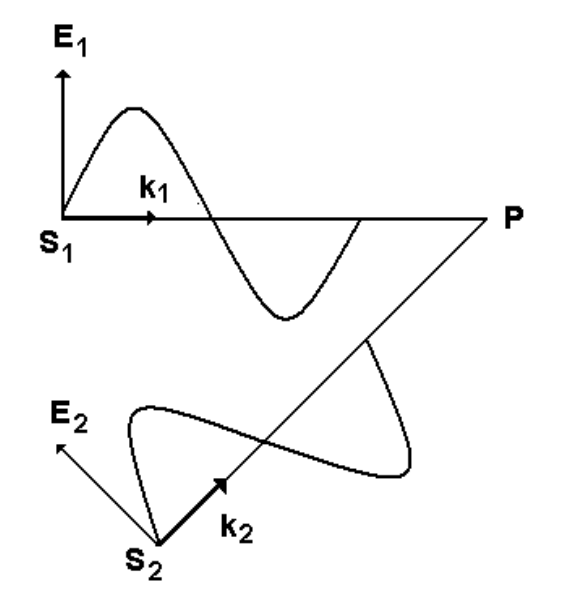
\includegraphics[width=0.3\textwidth]{Images/theory/interference.png}
    \caption{Two waves, $S_1$ and $S_2$, interfering}
    \label{fig:interference}
\end{figure}
Of Figure \ref{fig:interference}, one can conclude that the resulting wave, $\textbf{E}$ must be the sum of the two vectors interacting, $\textbf{E} = \textbf{E}_1 + \textbf{E}_2$. This applies to the resulting phase difference too, which thereby can be retrieved from (\ref{eq:2intphase}): $\sigma = \textbf{k}_1\cdot \textbf{r}_1 - \textbf{k}_2\cdot \textbf{r}_2 + (\xi_1 - \xi_2)$. Now, the intensity of the final wave can be found by multiplying this resulting wave-vector, $\textbf{E}$, with its conjugate, $\textbf{E}^*$: 

\begin{equation}
    I = \textbf{E} \cdot \textbf{E}^* = \textbf{E}_{01}^2 + \textbf{E}_{02}^2 + 2\textbf{E}_{01}\cdot \textbf{E}_{02} cos(\sigma)
    \label{eq:two-wave-intensity}
\end{equation}
\\\\
The intensity in the equation above, (\ref{eq:two-wave-intensity}), represents constructive interference at its maximum, whenever $cos(\sigma)$ is equal to 1, and expresses destructive interference at its minimum, when $cos(\sigma)$ equals -1. Constructive interference is hence present when the phase shift, $\sigma$ is expressed as:

\begin{equation}
    \sigma = 2 n \pi,
    \label{eq:maks}
\end{equation}

where n is the spectral order, a positive or negative integer. 
\\\\
Now, let us apply this to N number of waves, with several wave sources, up to $S_N$, as displayed in the figure below, Figure \ref{fig:Ninterference}.
\begin{figure}[h]
  \centering
    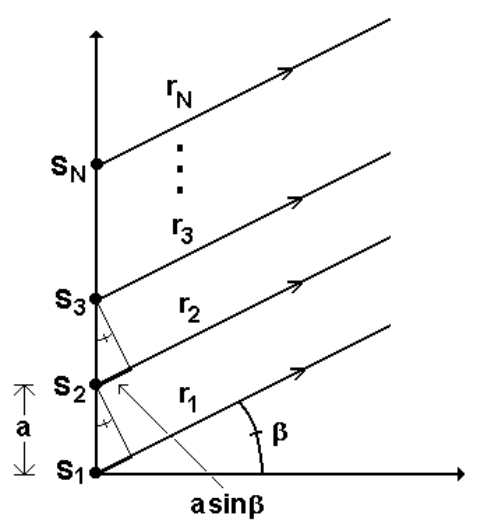
\includegraphics[width=0.3\textwidth]{Images/theory/Ninterference.png}
    \caption{N number waves propagating with a constant distance a}
    \label{fig:Ninterference}
\end{figure}
\\\\
The N waves are emitted by $S_N$ coherent and monochromatic sources separated by a distance, $a$. As the waves are coherent, the phase difference between the waves are constant. This means that the second term in (\ref{eq:2intphase}) can be ignored because $\xi_1$ = $\xi_2$ = ... = $\xi_N$. The phase difference is thus only due to the path difference between the waves, $\sigma = \textbf{k} \cdot \textbf{r}$. Of Figure \ref{fig:Ninterference}
$\textbf{r}$ can be retrieved as $a sin (\beta)$, while $k= \frac{2 \pi}{\lambda}$. Combining this with (\ref{eq:maks}), $\textit{the grating equation}$ is found: 
\begin{equation}
    n \lambda = a sin(\beta)
    \label{eq:transgrating}
\end{equation}

\section{Diffraction} \label{sec:diffraction}
While interference is a result of individual sources interacting with each other, diffraction is present when a wave is distorted by an external object, with a comparable dimension to the wavelength of the wave. Figure \ref{fig:diffraction} exemplifies diffraction with a port entrance wall as the external object. 
\begin{figure}[h]
    \centering
    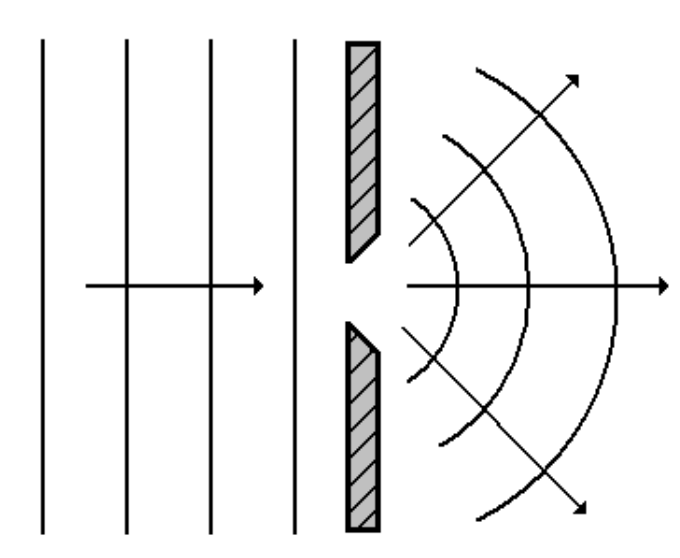
\includegraphics[width=0.3\textwidth]{Images/theory/diffraction.png}
    \caption{Diffraction as a result of waves hitting an entrance port}
    \label{fig:diffraction}
\end{figure}
\\\\
When the waves hit the external object in the figure above, a number of new waves originated from only one propagating wave, will be born. These children waves will, in turn, hit each other. This way, diffraction on the finite wave can be calculated as interference of the wave itself.

%TIL GRISM: 
%that the location of the intensity maxima for each order increases for increasing wavelength. This effect is the opposite of what happens with a prism, where there are no spectral orders and blue light is more refracted than red.

\subsection{Reflective Gratings}
The grating equation, (\ref{eq:transgrating}), assumes a grating transmitting light. The reflective grating, however, reflects the light. This grating can be thought of as a polished surface with parallel grooves - as shown in Figure \ref{fig:refgrating}. Between the grooves, parallel mirrors constitutes the grating, each mirror acting as a source of interference. 
\begin{figure}[h]
    \centering
    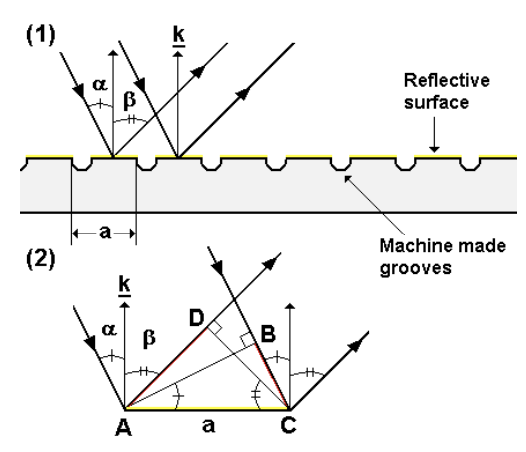
\includegraphics[width=0.4\textwidth]{Images/theory/refgrating.png}
    \caption{(1) Reflective
grating. (2) Resulting rays, where the red lines describe the associated phase difference}
    \label{fig:refgrating}
\end{figure}
\\\\
As explained in Section \ref{sec:light}, the phase difference of waves propagating from coherent sources is $\sigma = \frac{2 \pi}{\lambda} \cdot \textbf{r}$. Of the figure above, Figure \ref{fig:refgrating}, $\textbf{r}$ can be calculated as $(BC - (-AD))$. Based on this, the phase difference as a function of reflective grating can be presented as:
\begin{equation}
    \sigma = \frac{2 \pi}{\lambda}(BC + AD) = \frac{2 \pi}{\lambda} (a sin(\alpha) + a sin(\beta))
\end{equation}
\\\\
At maximum intensity (\ref{eq:maks}), the reflecting grating equation is found:
\begin{equation}
    n \lambda = a (sin(\beta) + cos(\alpha))
    \label{eq:refgrating}
\end{equation}
\\\\
Once again, n is the spectral order. $\alpha$ is the incident angle, and $\beta$ represents the diffracted angle of the grating.

\subsection{Angular Dispersion}
Angular dispersion is a measure of how the diffracting waves are spread, per unit wavelength. The angular dispersion of a grating is defined as $d\beta/d\lambda$. This can be derived by differentiating the grating equation, (\ref{eq:refgrating}). 
\begin{equation}
    \frac{d\beta}{d\lambda} = \frac{n}{a cos(\beta)}
    \label{eq:angdisp}
\end{equation}

\section{The GRISM} \label{sec:grism}
A GRISM is a combination of a grating and a prism - hence the name. The GRISM is a prism stacked in series with a transmission grating, as can be observed in Figure \ref{fig:grism} below.
\begin{figure}[H]
    \centering
    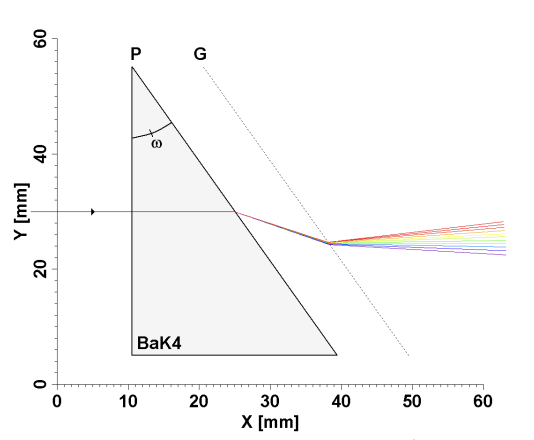
\includegraphics[width=0.5\textwidth]{Images/theory/GRISM.png}
    \caption{Light passing through a prism, P, dispersing blue light more than red, and a grating, G, diffracting red light more than blue}
    \label{fig:grism}
\end{figure}
\\\\
\noindent
For a grating, the intensity maximum for each spectral order, n, increases with increasing wavelength. A prism however, have no spectral orders and refracts blue light more than red. The net effect is a compact spectrum able to obtain a straight through center wavelength, parallel to the optical axis of the system. This on-axis effect, makes it easy to stack additional optics in both ends - the front and the back side of the GRISM. Due to absence of off-axis effects, image quality is preserved.
\\\\
When calculating the angular dispersion of a GRISM, the result is equal to the angular dispersion of a grating (\ref{eq:angdisp}), except for one additional term. This turns out to be a non-negative term, implying that the GRISM has an increased angular dispersion compared to a grating alone.

\section{The Behavior of Light in Air}
Light in air behaves differently than in water. In air, the light will not be attenuated, which means that the reflection can be expressed by the light intensity, $I_ {\lambda}$ (\ref{eq:int}), describing the colors observed on the object.
\begin{equation} \label{eq:int}
    I_ {\lambda} (L, z) = \frac{S \cdot \kappa_{\lambda}\cdot cos^{3}\cdot (\alpha)}{z^2}
\end{equation}
\\\\
In (\ref{eq:int}), $I_{\lambda}$ represents the light intensity at a given wavelength, lambda, while S is the light source. L is the distance between the object and the viewpoint, while z describes the distance from the object to the light source. Furthermore, $\kappa_{\lambda}$ describes the reflectance ratio of the object's surface at a given wavelength, $\lambda$. $\alpha$ is the angle between the ray vector from the light source and the normal vector of the object surface. Figure \ref{fig:reflectance} illustrate this with a simple set-up.
\begin{figure}[H]
\centering
  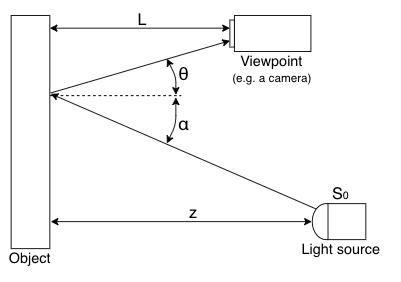
\includegraphics[width=8cm]{Images/theory/reflectance.png}
  \caption{Light refraction in liquid}
  \label{fig:reflectance}
\end{figure}
\\\\
\noindent
However, these properties cannot be directly drawn when do the same underwater. In water, light attenuation will be present and affect how the light is reflected. In addition, light is possibly scattered at stages resulting in a change in the direction. In the figure, these stages are leaving the light source and after hitting the object.\todo{marreg1-kilde, side 83} This will be elaborated in the following sections.

\section{The Behavior of Light in Water}\label{lightinwater}
%The light intensity decreases with the distance from objects in water by light attenuation depending on the wavelength of light. Red light decreases easier than blue light in water [E. O. Hulburt: “Optics of Distilled and Natural Water,” Journal of the Optical Society of America, Vol.35, pp.689–705, 1945].
The reason why the color of objects underwater differ from when in air, is that the light intensity, in water, decreases with the distance (r) to the object. This is, as mentioned, due to light attenuation, which again depends on the wavelength of the light. %([E. O. Hulburt: “Optics of Distilled and Natural Water,” Journal of the Optical Society of America, Vol.35, pp.689–705, 1945].) 
\\\\
From Figure \ref{fig:lightinwater}, it can be observed that the intensity of the different colors decreases differently, even at the same distance, r. If the light source is 2 m away, red light will shine at half intensity, while blue light remains close to unchanged. At a distance of 20 meters, blue light will brighten at half-intensity. In this case, red and orange color will disappear.
%Color Registration of Underwater Images for Underwater Sensing with Consideration of Light Attenuation
%https://ieeexplore.ieee.org/stamp/stamp.jsp?tp=&arnumber=4209801
\begin{figure}[H]
\centering
  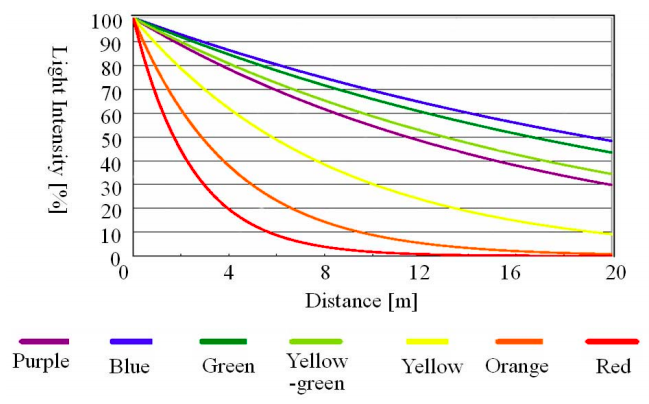
\includegraphics[width=9.5cm]{Images/theory/intensity.png}
  \caption{Light intensity in water.}
  \label{fig:lightinwater}
\end{figure}
\\\\
\noindent
As shown in the figure \ref{fig:lightinwater}, the light intensity decreases exponentially. The figure, is based on the following equation for the light source, S. 

\begin{equation} \label{eq:source}
S_{\lambda} (z) = S_0 \cdot exp (-c_{\lambda} \cdot r)
\end{equation}
\\\\
In (\ref{eq:source}), $S_{\lambda}$ describes the light intensity at wavelength $\lambda$, while $S_0$ is the intensity at the light source. Furthermore, r describes the distance between the light source and the viewpoint, while $c_{\lambda}$ is the attenuation coefficient of the wavelength $\lambda$, illustrated by Figure \ref{fig:attcoeff}.
\\\\
By taking the attenuation coefficient, $c_{\lambda}$, into consideration, the light intensity in water can be expressed by the following similarity. 

\begin{equation} \label{eq:intw}
    I_ {\lambda} (L, z) = \frac{S \cdot \kappa_{\lambda}\cdot cos^{3}\cdot (\alpha)}{z^2} \cdot exp \left(-c_{\lambda}\left(\frac{z}{cos(\alpha)}\frac{L}{cos(\theta)}\right)\right)
\end{equation}
\\\\
Interpreting (\ref{eq:intw}), the intensity of light decreases when $c_{\lambda}$ increases. If $c_{\lambda} = 0$, meaning the light attenuation not being present, the resulting intensity becomes the same as the light intensity in air, (\ref{eq:int}). 

\begin{figure}[H]
\centering
  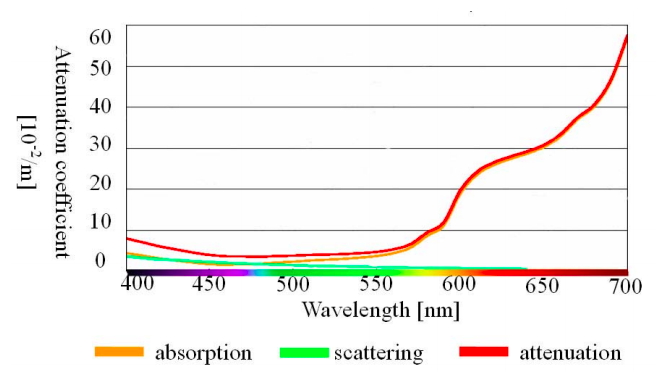
\includegraphics[width=9.5cm]{Images/theory/attcoeff.png}
  \caption{Attenuation coefficient}
  \label{fig:attcoeff}
\end{figure}


%Attenuation coefficient consists of absorption coefficient and scattering coefficient, because light attenuation consists of light absorption and light scattering. Attenuation coefficient of water changes very much with the wavelength of light. Consequently, observed colors changes in underwater environments.


%Stereo Measurement of Objects in Liquid and Estimation of Refractive Index of Liquid by Using Images of Water Surface
%http://www.robot.t.u-tokyo.ac.jp/~yamashita/paper/B/B047Final.pdf
%\noindent
%Note that if cameras and objects are in the different condition where the refraction index differs from each other, several problems occur and a precise measurement cannot be achieved.
\vspace{1.6cm}
\noindent
However, the analysis above applies to visual light. What happens when exploring a larger part of the wave spectra? As it turns out, the earlier viewed trends are no longer linear.
\\\\
%http://www1.lsbu.ac.uk/water/water_vibrational_spectrum.html
Water absorbs wavelengths covering a wide range of electromagnetic radiation. For light with wavelengths larger than 200 nm, this absorption is due to rotational transitions and intermolecular vibrations. As the H2O-molecule has a particularly small moment of inertia on rotation, a rich vibrational-rotational spectrum appears, sometimes containing millions of absorption lines. 
\\\\
The water absorption spectrum is therefore very complex. The water molecule may vibrate in several ways, at several states affected by the environment. For the specific case of H2O, the absorption spectrum is displayed in Figure \ref{fig:absspec}. The spectrum may vary based on the condition of the water and placement of measurement - for instance whether one looks at the open sea or the coastal areas. However, the trends represented in the figure, should more or less remain. The spectrum clearly shows how the water absorption is at its lowest in visible light, making this range of wavelengths more optimal when detecting objects underwater. Near infrared light, on the other hand, will quickly disappear over short distances. This could result in large variations in the resulting spectral signatures, leaving a possibly non-representable set of data.

\begin{figure}[H]
    \centering
    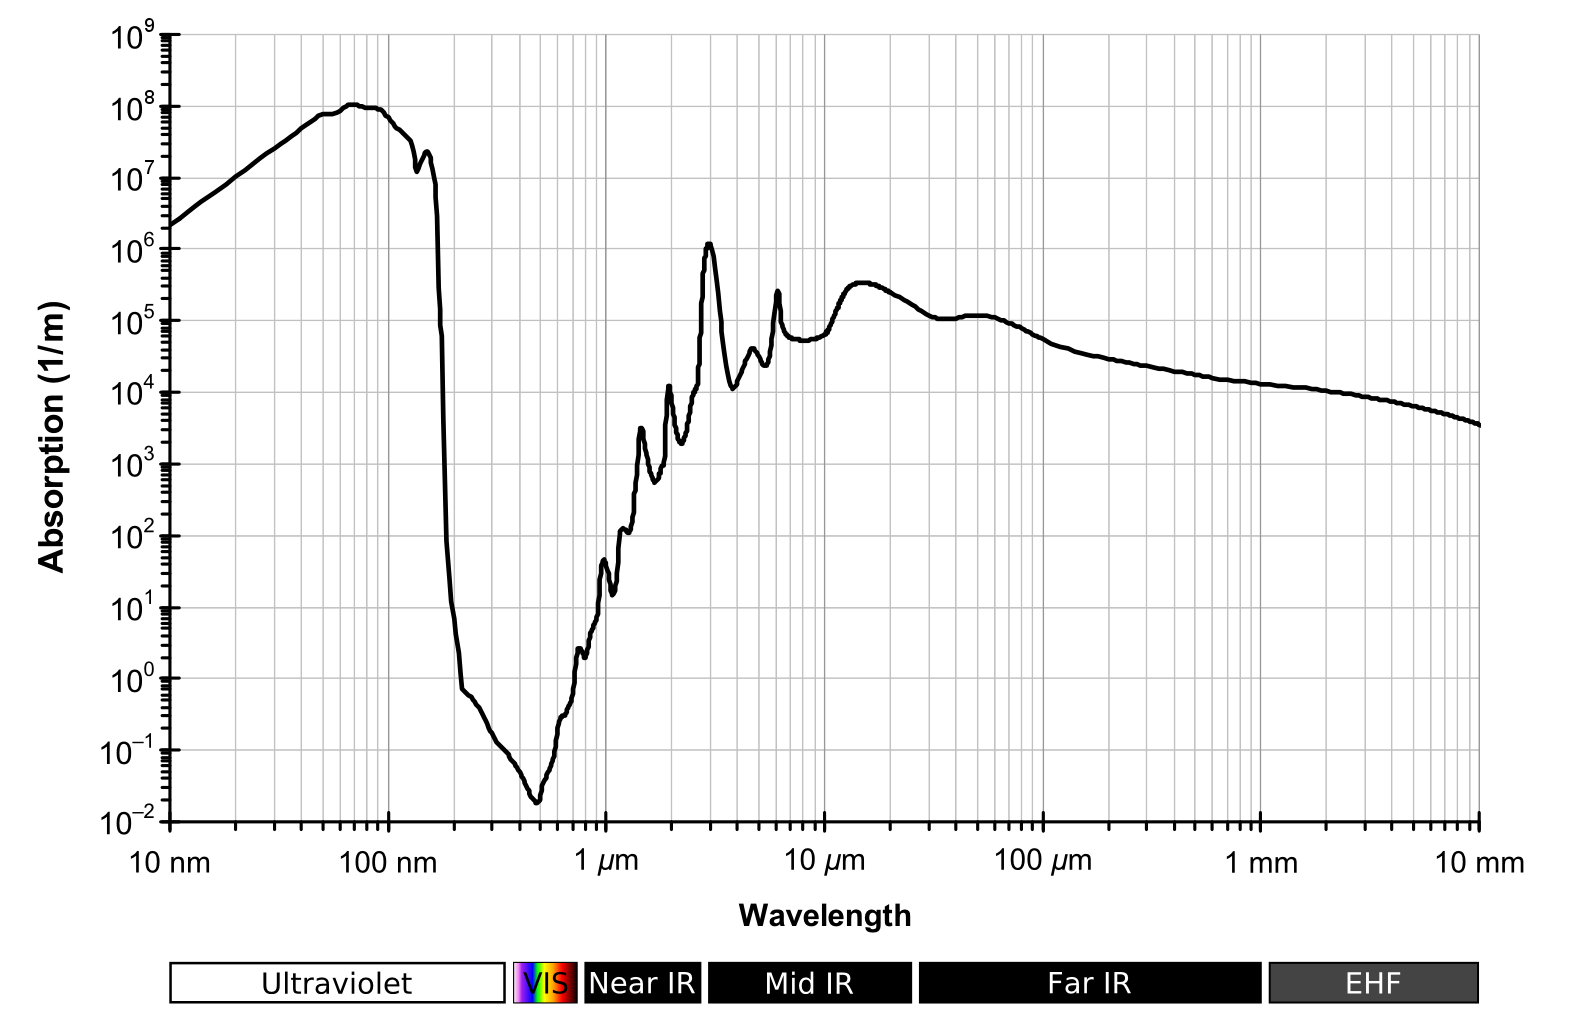
\includegraphics[width=8cm]{Images/theory/Absorption_spectrum_of_liquid_water.png}
    \caption{Absorption spectrum of liquid water}
    \label{fig:absspec}
\end{figure}


\begin{comment}
%PAPER: Identification and Classification of Plastic Resins using Near Infrared Reflectance PSpectroscopy: https://www.researchgate.net/publication/285330830_Identification_and_classification_of_plastic_resins_using_near_infrared_reflectance_spectroscopy

%https://oceanoptics.com/plastic-recycling-nir-spectroscopy/ Plastic Recycling with NIR Spectroscopy - denne inneholder signaturene til plast i NIR
%Another important observation in these experiments, is the condition of the microplastic used. The material is pure and white, making the results independent of color. 


Water absorption: 
%https://commons.wikimedia.org/wiki/File:Absorption_spectrum_of_liquid_water.png
This logarithmic (log-log) graph shows water’s absorption behavior at different colors wavelength. As seen in the graph, water absorption is minimised between 400 -600 nm


Light Transmission in the Ocean: http://www.waterencyclopedia.com/La-Mi/Light-Transmission-in-the-Ocean.html
https://manoa.hawaii.edu/exploringourfluidearth/physical/ocean-depths/light-ocean
\end{comment}


\section{Properties of Photons}\label{sec:photons}
%https://snl.no/foton
All electromagnetic radiation, including light, consists of photons. Just as all objects that have mass are built up of atoms, massless light rays are the result of many energy-consistent photons. In order to the determine the amount of light (number of photons) actually passing through a spectrometer, etendue and throughput must be defined. 

\subsection{Etendue}\label{sec:etedue}
The amount of light detected by the instrument is described by the acceptance area or the field of view photons can travel into. Etendue is the maximum geometric extent allowing traveling photons and thereby characterizing an optical system's ability to accept light. Figure \ref{fig:etendue} is an illustration showing how to review etendue. 

\begin{figure}[H]
    \centering
    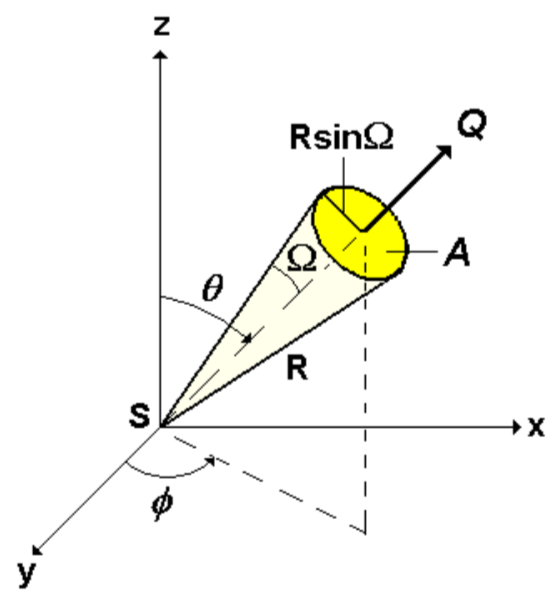
\includegraphics[width = 6cm]{Images/theory/etendue.png}
    \caption{Set-up explaining Etendue}
    \label{fig:etendue}
\end{figure}
\\\\
\noindent
S describes the emitting source of light, while Q is the solid angle of which the light propagates into (or out of). By definition, etendue, $G$ is found by $G := \int\int dS dQ$. For a simple spectrometer like the one viewed in this assignment, $G = S \cdot Q = \pi S sin^2(\Omega)$.
\\\\
An instrument is defined to be optimally constructed when the instrument can ensure an absence of light loss. This requires a constant etendue throughout the instrument without any reduction from geometrical blocking. The latter implies the similarity $G_2 = G_3$, or $\pi S_2 sin^2(\Omega_2) = \pi S_3 sin^2(\Omega_3)$. The relations between the latter properties will be easier to understand when after looking at the figure describing a spectrometer, Figure \ref{fig:sysopt} in Section \ref{sec:sysopt}. 
\\\\
The optimal exit slit width can be calculated from holding the etendue constant through the elements involved - starting at the entrance slit eventually reaching the exit slit. From the entrance slit, the etendue can be expressed by 
\begin{equation}
    G_2 = \frac{G_A cos(\alpha)}{f_2^2} \cdot w \cdot h
    \label{eq:etenentr}
\end{equation}

Similarly can the etendue from the exit slit be described as follows

\begin{equation}
    G_3 = \frac{G_A cos(\beta)}{f_3^2} \cdot w' \cdot h'
    \label{eq:etenexit}
\end{equation}
\noindent
w and h is the entrance width and height, while w' and h' explains similar properties at the exit slit. $G_A cos(\alpha)$ and $G_A cos(\beta)$ defines the illuminated area of the grating as seen from the entrance and exit slit, respectively. Using similarity of form, $h \cdot f_2 = h' \cdot f_3$. Conducting calculations using all of the above, the resulting optimal exit slit width can be found by following similarity.
\begin{equation}
    w' = \frac{cos(\alpha)}{cos(\beta)}\cdot \frac{f_3}{f_2}\cdot w
    \label{eq:exit}
\end{equation}
\\\\
\noindent
Expressing the exit slit as a function of the entrance slit, reveals useful information on the spectral bandpass and resolution discussed in Section\ref{sec:bp}. 

\subsection{Flux}
Flux is defined as the number of photons traveling into a solid angle Q, when emitted from a source, $S$, per unit time [sec]. By this definition, flux $\Phi$ can be expressed as:
\begin{equation}
    \Phi = \frac{#photons}{s}
    \label{eq:flux}
\end{equation}
Flux can describe both the light intensity and the radiance. This intensity, $I$ is can be found by computing the flux, $\Phi$ per unit solid angle [$sr$]:
\begin{equation}
    I = \frac{\Phi}{Q} = \frac{#photons}{sr \cdot s}
    \label{eq:i}
\end{equation}
The radiance, $B$ is the intensity through a unit surface area, A [cm], where A is the yellow area in Figure\ref{fig:etendue}. Given (\ref{eq:flux}), $B$ can also be described as the flux of photons per unit area and solid angle.
\begin{equation}
    B = \frac{I}{A} = \frac{#photons}{cm^2 \cdot sr \cdot s}
    \label{eq:b}
\end{equation}
\\\\
Applying the terms above to the definition of etendue, the photon flux through the geometric extent being the etendue, can be described as a function of etendue and radiance. 
 \begin{equation}
     \Phi := B\cdot G
     \label{eq:flux2}
 \end{equation}
As will be shown in Section \ref{sec:tput}, (\ref{eq:flux2}) is useful when evaluating the fluxes of photons entering and leaving a spectrometer.

\subsection{Throughput} \label{sec:tput}
Throughput defines the amount of flux hitting the detector (CCD) at the end of the spectrometer. Simply put, throughput is the usable flux. From (\ref{eq:etenentr}) and (\ref{eq:etenexit}), the following similarities can be stated. Assuming that $B_2$ is the total radiance of the entering source of light, (\ref{eq:fluxinn}) describes the flux entering the entrance slit, while (\ref{eq:fluxut}) describes the flux exiting the spectrometer system. 

\begin{equation}
    \Phi_2 = B_2 \cdot G_2 = B_2 \cdot \frac{G_A cos(\alpha)}{f_2^2} \cdot w \cdot h
    \label{eq:fluxinn}
\end{equation}

\begin{equation}
    \Phi_{\lambda} = B_{r} \cdot G_3 = B_{\lambda}\cdot E_{\lambda}^n \cdot T_{\lambda} \cdot \frac{G_A cos(\beta)}{f_3^2} \cdot w' \cdot h'
    \label{eq:fluxut}
\end{equation}
\noindent
In (\ref{eq:fluxut}), $B_{r}$ describes the remaining radiance at the end of the spectrometer, and includes the spectral radiance, $B_{\lambda}$,  multiplied with reducing factors due to loss. $E_{\lambda}^n$ describes the efficiency of the used grating at spectral order n. $T_{\lambda}$ is a factor describing losses due to geometry of the components in the spectrometer. For an optimal spectrometer with an unrealistically efficient gradient, both $E_{\lambda}^n$ and $T_{\lambda}$ are equal to 1.

\section{Inherent Optical Properties (IOP)}
%http://iopscience.iop.org/article/10.1088/0034-4885/36/12/002/pdf
%noe av dette har blitt sagt i hyp også:
When retrieving an optical fingerprint it is important to know the optical properties impacting the resulting signature. There are mainly three physical processes reducing the energy of light on its way to reaching the receiver. The OOI (the materials or the compositions of materials) will absorb, scatter and reflect light of different portions of the visible spectrum. This way, the material of the OOI and the wavelength will affect the properties of these processes. 
\\\\
Scattering, absorption and reflection are all results of photons interacting with the OOI. 
%http://www.oceanopticsbook.info/view/overview_of_optical_oceanography/inherent_optical_properties
\subsection{Absorption} \label{sec:abs}
During the photon-OOI interaction, the energy of the photon can be converted to another form, leaving the photon to disappear and hence the light to be absorbed. 
\\\\
%https://www.physicsclassroom.com/class/light/Lesson-2/Light-Absorption,-Reflection,-and-Transmission
Atoms and thereby molecules contain elections. Given the specific atom, these electrons hold a specific natural frequency. Whenever light hits these molecules, the electrons in that molecule will be given a vibrating motion if the energy of the photon match the gap between the energy levels in the targeted atom. Then the frequency of the light is equal to the electrons natural frequency. The creation of vibration is a result of energy usage – energy taken from the photons in the light. This way, the electrons absorb the energy of the light by turning it in to vibration energy, which cannot be converted back to light. 
\\\\
Different atoms will absorb light at different wavelengths, because they hold different sets of natural vibration frequencies. 

%{pluss coeff og internsitets-likn?}
%{pluss figur?}

\subsection{Scattering}
During the photon-OOI interaction, the photon might either change its direction, its energy or both. Either of these processes are called scattering. %http://iopscience.iop.org/article/10.1088/0034-4885/36/12/002/pdf 
More precisely, scattering can be defined as \textit{the change in direction of light flux produced by individual parcels of particulate matter called ‘scatterers’}. This means that light, or other moving particles, are forced to deviate from the straight trajectory they were on to being with, due to the collision between the light wave and the OOI. 
\\\\
%http://www.oceanopticsbook.info/view/overview_of_optical_oceanography/inherent_optical_properties 
As mentioned, these inherent optical properties are again dependent on many other properties. Different materials absorb and scatter very much differently as a function of wavelength. If comparing to particles with the same volume, they will scatter light differently if are of different shapes. Similarly, particles with exact same shape will scatter light differently whenever the volume of the particles differ. A change in the material, size or shape (or the composition of them) will give different IOPs. 
\\\\
In the ocean, the physical characteristics of the OOI are highly affected by the surroundings, implying that the IOPs are too. As an example, a change in the concentration of plankton or being in coastal waters instead of the open ocean, will contribute to a significant change in both the resulting absorption and scattering. 


\subsection{Spectral Reflectance}\label{sec:specref}
Light reflection from an object means that waves of light hitting the surface of the object is sent back from the surface. Reflection happens when the wavelength of the light waves do not match the natural vibration frequencies of the hit object. Whenever such waves of light strike the object, the electrons in the atoms of the object will vibrate. However, this is not the same type of vibration as the one discussed above (Section \ref{sec:abs}). Now, the electrons vibrate in small amplitudes for no more than brief periods of time. This causes the energy to re-emit as a wave of light, rather than turn into vibration energy an be absorbed at resonance vibration. 
\\\\
\begin{comment}
%Underwater hyperspectral imaging: a new tool for marine archaeology 2018, ØYVIND ØDEGÅRD,1,2,* AKSEL ALSTAD MOGSTAD,3 GEIR JOHNSEN,3 ASGEIR J. SØRENSEN, AND MARTIN LUDVIGSEN1
Raw data consists of more than upwelling radiance reflected from the object. Reflections from the water column, ambient light and noise sensors are all parts of the data collected. However, the spectral reflectance reference is independent of the illumination and the water column properties. 
\end{comment}
%Underwater hyperspectral imagery to create biogeochemical maps of seafloor properties 2013, G. JOHNSEN, NTNU
The spectral reflectance, also called the optical fingerprint can be described as a percentage of the light amount reflected off an object at each wavelength. As mentioned, different objects absorb and reflect different wavelengths. In plants, red and blue wavelengths are highly absorbed, leaving the reflected color to be more or less green. Mathematically speaking, the spectral reflectance, $R(\lambda)$ is upwelling irradiance coming off the object, $Lu(\lambda)$, divided by the spectral downwelling irradiance towards the object, $Ed(\lambda)$.
\\\\
%The use of underwater hyperspectral imaging deployed on remotely operated vehicles – methods and applications - geir og asgeir
\begin{equation} \label{eq:specref}
    R(\lambda) = \frac{Lu(\lambda)}{Ed(\lambda)}
\end{equation}
\\\\
Where $Lu(\lambda)$ denotes the raw data of the object, including signature from light source, while $Ed(\lambda)$ is the spectral radiance from measurements of spectrally neutral reflectance standard.
\\\\
Note: For (\ref{eq:specref}) to hold true, all surfaces are assumed to behave like Lambertian reflectors, meaning that the reference surface has a perfectly diffuse/matte property. This ensures that the radiant intensity, regardless of the reflected direction, is proportional to the cosine of the angle of the surface's normal. This is known as Lamberts Cosine law. 
%det siste er tatt fra TTK20-heftet


%The use of underwater hyperspectral imaging deployed on remotely operated vehicles – methods and applications - geir og asgeir

\section{System Optics} \label{sec:sysopt}
Rays travelling through a spectrometer can be described by an optical diagram like the one presented below in Figure \ref{fig:sysopt}.
\begin{figure}[H]
    \centering
    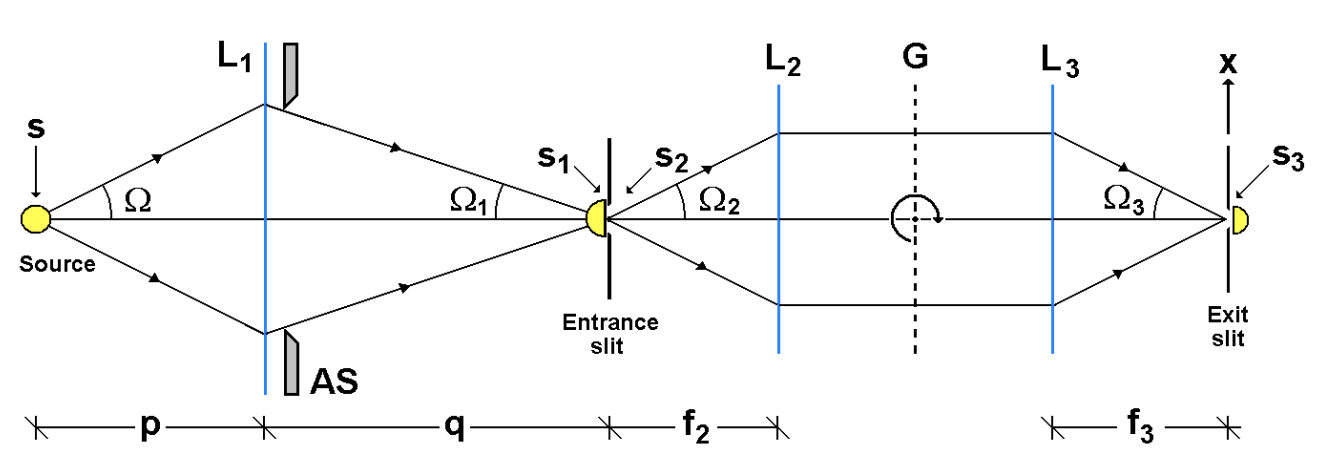
\includegraphics[width = 12cm]{Images/theory/sysop.png}
    \caption{Optical diagram of a Spectrometer}
    \label{fig:sysopt}
\end{figure}
\noindent
From the figure, one can extract $S$ as the source of light. $S$ illuminates the front lens, $L_1$, with the angle $\Omega$. Furthermore the front lens focuses the light onto the entrance slit, resulting in the imaged area, $S_1$. $G$ is the grating, either transmitting or reflecting, in which $L_2$ collimates with light passing through the entrance slit area, $S_2$, at an angle  $\Omega_2$. The diffracted beam of light from the grating is then focused onto the exit slit by $L_3$, as a function of wavelength. This makes $S_3$ the area of the diffracted entrance slit image. 
\\\\
$f_2$ and $f_3$ are the corresponding focal lengths of $L_2$ and $L_3$. Note that as long as $L_1$, $L_2$ and $L_3$ are able to focus or collimate the beam of light, they can be mirrors instead of lenses. 


\subsection{The Spectral Bandpass and Resolution} \label{sec:bp}
%https://www.horiba.com/en_en/bandpass-resolution/
Both spectral bandpass and resolution characterize the ability the instrument has to separate adjacent spectral lines. This way, the bandpass defines the spectral interval to be isolated. This is assuming the light source is continuum. As will be shown below, the bandpass is mainly dependent on  the width of the grating, entrance and exit slit widths and the spatial resolution of the CCD. 
\\\\
The isolated spectral interval (bandpass) can be found from the recorded Full Width at Half Maximum (FWHM) of a monochromatic spectral line. In reality, there are no perfect spectrometer. This is why the bandpass is approximated to FWHM. Figure \ref{fig:bp} shows the effect of spectral resolution of a monochromatic line. As displayed, the bandpass at wavelength $\lambda_0$ can be found at half intensity, $B$. 

\begin{figure}[H]
    \centering
    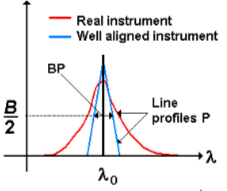
\includegraphics[width=5cm]{Images/theory/bp.png}
    \caption{Spectral resolution of monochromatic line}
    \label{fig:bp}
\end{figure}
\todo{lage en finere skisse}
\noindent
Note that the assumption of a monochromatic spectral line does not restrict to only one line. Any spectral structure can be considered as the sum of infinite single monochromatic lines at different wavelengths.
\\\\
The spectral bandpass can then be calculated as the wavelength distribution along the x-axis multiplied by the exit slit width. This wavelength distribution is called \textit{the linear dispersion}, and is defined as $d\lambda/dx$. Using the angular dispersion from (\ref{eq:angdisp}) and the similarity $dx = f_3 d\beta$, the spectral bandpass can be calculated. As known from (\ref{eq:exit}) in Section\ref{fig:etendue}, the exit slit width, $w'$ is dependent on the entrance slit width, $w$ through $w' = \frac{cos(\alpha)}{cos(\beta)}\cdot \frac{f_3}{f_2}\cdot w$.

\begin{equation}
    %\begin{split}
    FWHM = \frac{d\lambda}{dx} \cdot w'\hspace{0.5cm}
    = \frac{d\lambda}{d\beta} \frac{d\beta}{dx}\cdot w' \hspace{0.5cm}
    = \frac{a cos(\beta)}{n} \frac{1}{f_3}\cdot w' \hspace{0.5cm}
    = \frac{a cos(\alpha)}{n\cdot f_2}\cdot w
    %\end{split}
    \label{eq:bp}
\end{equation}
\\\\
\noindent
In (\ref{eq:bp}), $\alpha$ is the incident angle and $\beta$ is the diffracted angle. $f_2$ and $f_3$ are, as mentioned, the focal lengths associated with the lenses $L_2$ and $L_3$ respectively.


%\subsection{Bandpass and Resolution}
\subsection{The GRISM Spectrograph}
In section \ref{sec:grism}, the GRISM, and how it could obtain a straight through center wavelength parallel to the optical axis, was elaborated. Therefore, using a GRISM as the dispersive element is popular when designing a spectrometer. Figure \ref{fig:grismspec} shows a typical 3D configuration of a GRISM spectrograph in hyperspectral image mode, illustrating the basic elements of hyperspectral imaging. Of the illustration, one can observe how the elements are stacked at the right next to each other (on axis), supporting the previous stated properties of the GRISM. This on-axis design reduces geometrical aberrations and thereby improves the resolution. 
\\\\
Similar to the spectrometer already discussed above (section \ref{sec:sysopt}), the front lens focuses light onto the entrance slit $S_1$, while $L_2$ collimates the GRISM. The diffracted light is then focused into the image detector (CCD), by $L_3$. 

\begin{figure}[H]
    \centering
    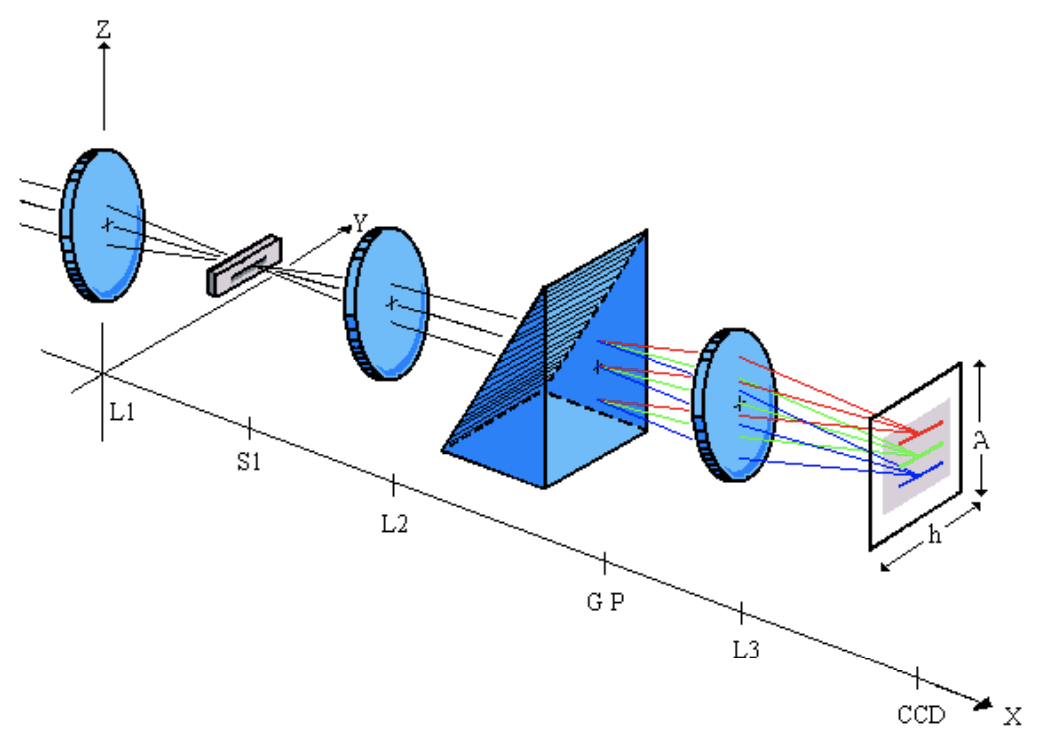
\includegraphics[width = 12cm]{Images/theory/grismspec.png}
    \caption{The GRISM spectrograph}
    \label{fig:grismspec}
\end{figure}


\chapter{Imaging} %imaging
\label{chap:theory2}
%Imaging Process
%Denne skal jeg få tilsendt av Asgeir

This chapter illuminates the imaging process - from the commonly known digital image to the hyperspectral image, containing an additional dimension of information improving the resolution of the image. In addition to the hyperspectral camera, SINTEF has developed a silhouette camera, possibly covering information the hyperspectral camera cannot retrieve.


\section{The Digital Image}
%evt Fysikken bak bildet 
%Info hentet fra bok: techniques and applications of hyperspectral image analysis
From the mid-20th century, images have been stored in digital format (Geladi and Grahn, 2000). A digital image is an array of rows (i) and columns (j) consistent of i x j gray-values. A gray-value, better known as an intensity or a pixel, is simply one of many small squares in an image. If the image is to consist of colors however, a third dimension is needed. This dimension is characterized as the depth, and can be found as the height in Figure \ref{fig:pogv}b). The depth is three layers deep, consisting of red, green and blue. What was previously a gray pixel is now a voxel illustrated in \ref{fig:pogv}b), with triplet of red, green and blue - each of which contains different information. Note that the height of the voxel is almost undetectable, as the voxel only consists of the tiniest distinguishable element of a 3D object.
\\\\
However, if the interval separating the layers is chosen to be a shorter wavelength, the number of layers will increase. The resulting image is then called a multivariate image, illustrated in Figure \ref{fig:pogv}c). If k denote the depth dimension and thus determine the number of wavelengths which in turn will constitute the number of layers, the resulting array will be of the size i x j x k.
\\\\
For the human eye to be able to perceive a color image, only three wavelengths/layers are needed, namely red, green and blue. It therefore rarely makes sense to create multiple layers unless the goal is to capture information the eye cannot see. This is where hyperspectral imaging enters the playing field, which by definition has more than 100 layers and can express each pixel as a spectrum.

\begin{figure}[H]
  \newcommand*\FigVSkip{0.5em}
  \newcommand*\FigHSkip{0.1em}
  \newsavebox\FigBox
  \centering
  % Top image is centered, so no need to get width
 \sbox{\FigBox}{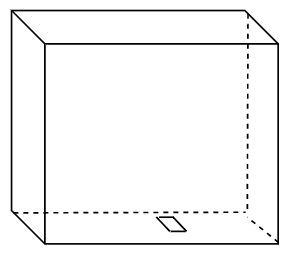
\includegraphics[scale=0.4]{Images/theory/pixel.png}}
  \begin{minipage}{\wd\FigBox}
    \centering\usebox{\FigBox}
    \subcaption{a) Pixel}
  \end{minipage}
    % Top image is centered, so no need to get width
 \sbox{\FigBox}{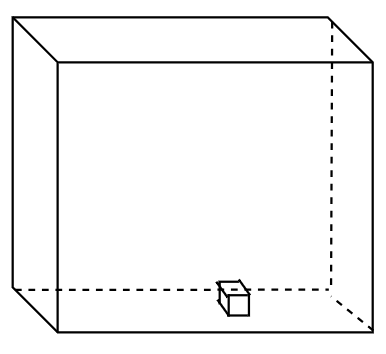
\includegraphics[scale=0.29]{Images/theory/voxel0.png}}
  \begin{minipage}{\wd\FigBox}
    \centering\usebox{\FigBox}
    \subcaption{b) Voxel}
  \end{minipage}
  % Save first image in a box to get the width
  \sbox{\FigBox}{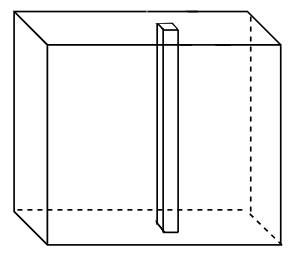
\includegraphics[scale=0.4]{Images/theory/voxel.png}}
  \begin{minipage}{\wd\FigBox}
    \centering\usebox{\FigBox}
    \subcaption{c) Multivariate Image}
  \end{minipage}\hspace*{\FigHSkip}
  % Save second image 
  \caption{Pixel, Voxel and Multivariate Image}
  \label{fig:pogv}
\end{figure}

\vspace{1.3cm}
\section{Hyperspectral Imaging}
%Info hentet fra yt
In order to study the reflecting light from the target, a spectrometer is needed. A spectrometer is an instrument that splits the incoming light into a spectrum. Measuring this reflectance spectra is the most common way to use hyperspectral imaging.
\\\\
Hyperspectral imaging uses a hyperspectral camera (imaging spectrometer) to collect spectral information. As mentioned, the difference between a hyperspectral image and a regular photo, is that the hyperspectral camera measures hundreds of thousands of spectra instead of single spectrum, creating not only a multispectral image, but a hyperspectral image. In contrast to multispectral imagers, which are sensitive in only a few selected wavebands, hyperspectral imagers (HI) measure the spectral reflectance per image pixel of the particular OOI, leaving a complete reflectance spectrum for each pixel in the image. %(Development of hyperspectral imaging as a bio-optical taxonomic tool for pigmented marine organisms - geir)

\subsection{On a Detailed Level}
%The Spatial Resolution
In detail, a spectrograph, illustrated in Figure \ref{fig:grismspec}, generates images from the entrance slit, as a function of wavelength (color). The amount of images detected by the CCD at the exit slit, is dependent on the entrance slit width and the element’s ability diffract the colors. The width of the exit slit being dependent on width of the entrance slit, was derived in (\ref{eq:exit}) in Section \ref{sec:etedue}, describing optimal etendue. A large amount of detected images at the exit slit will directly improve the spectral resolution of the instrument. The resulted image recorded by the CCD is called a spectrogram (an illustration of a spectrogram can be found as the last element in Figure \ref{fig:grismspec}). The spectrogram contains both spectral and spatial information and can be described by the intensity distribution and position along the slit. 
\\\\
However, the information retrieved is information about the covered area of the target object, which is nothing but a very thin track covering only a small part of the object. In order to obtain the object's full spatial extent, the entire object surface needs to be sampled. 
\\\\
Now, how can this be done? The recording instrument must be moved relative to the target. The velocity, $\nu$ of the instrument is crucial, as the instrument will under sample (miss samples of the target area) if the distance moved during readout time, $\tau$, exceeds the length of the measured area, $dx$ (displayed in Figure \ref{fig:spatialres}). This requirement is shown in (\ref{eq:req}).

\begin{equation}
    \nu \cdot \tau \leq dx
    \label{eq:req}
\end{equation}
This way, the image at the entrance plane moves across the slit so that the CCD can record spectrograms for each track of the object. This is called the push broom technique, which will be illustrated in Section \ref{sec:push}. When summarizing all samples, information on the continuous image can be retrieved.
\\\\
The required movement is based on the instrument and target moving relative to each other. Hence the movement can be created in two ways. Either the instrument can move, or the viewed target can be moved while keeping the imager still. If the target is located at a conveyor belt, it might be suitable to keep the instrument still. However, as mentioned, the magnitude of the relative movement is important. This means that if the conveyor belt is moving too fast, the instrument needs to move as well, in order to reduce the relative movement.
\\\\
Figure \ref{fig:spatialres} describes the situation where a hyperspectral imager is attached to an airplane moving at a velocity, $\nu$. In the illustration, $S$ is the slit, while $w$ is the associated width. $z$ describes the altitude above ground level. The front lens is denoted $L_1$, and has a focal length of $f_1$. 
\begin{figure}[H]
    \centering
    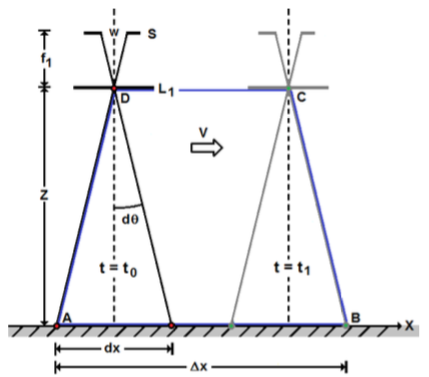
\includegraphics[height=7cm]{Images/theory/spatialres.png}
    \caption{Spatial resolution - Field of view (from a moving airplane)}
    \label{fig:spatialres}
\end{figure}
\noindent
It is common to believe that the spatial resolution is dependent on the number of pixels present along the wavelength axis of the detector. However, the amount of information is described by the number of spectral layers that hyperspectral imager can produce (illustrated as the height of the column in Figure \ref {fig:pogv}c)). The spectral layers define a dimension independent of the pixel-plane, only dependent on the bandpass (see section bandpass) and the spectral range of the instrument. Using similarity of form, $dx$ can be calculated from the lengths of the figure.
\begin{equation}
    dx = \frac{z \cdot w}{f_1}
    \label{eq:dx}
\end{equation}
During the exposure, the airplane has moved from the first state to the second. This distance can be calculated from the time spent at the constant velocity held: $distance = \nu \cdot (t_1 - t_0) = \nu \cdot \Delta t$. The spatial resolution becomes equal to the distance from A to B. Of the figure, this distance is observed as: 

\begin{equation}
    \Delta x = dx + \nu \cdot \Delta t
    \label{eq:spares}
\end{equation}
\noindent
(\ref{eq:dx}) shows how $dx$, an thereby also the spatial resolution, is connected to the spectral bandpass through the slit width, $w$, as described in Section \ref{sec:bp}. 

%Info hentet fra bok: techniques and applications of hyperspectral image analysis
 %oppsettene inkluderer lyskilde, et filtersystem som disperse the light into bands of wavelenghts, en sample. Hvis kilden inneholder et bredt lysspekter, kan man velge ut bølgelengder ved å bruke bandpass-filters etter ønske.


%The spectral information in every pixel creates a third dimension, providing a collection of data called a data cube. Now, how does this data differ from the data and images from other types of cameras? Digital camera, shoots the target in red, green and blue, in order to match the human vision. These camera leaves a combination of the three colors, which is what we can see with our eyes. This means that the information constituting the third dimension consists of nothing more than three colors, while the hyperspectral camera records hundreds of wavelengths. This way, the hyperspectral camera can collect more detailed information about the target, not only in visible light, but also in infrared and ultra violet. By combining different wavelengths, pixel by pixel, one can extract useful information about the properties of the target. 

\subsection{On an Environmental Level}
%Hyperspectral imaging and data analysis for detecting and determining plastic contamination in seawater filtrates, 2016,  Bert van Bavela
%http://journals.sagepub.com/doi/pdf/10.1255/jnirs.1212
\noindent
Concerning plastic, this translates to receiving information on both spatial location of plastic material, and the plastic materials composition. 
%Volent, Z., Johnsen, G., & Sigernes, F. (2007). Kelp forest mapping by use of airborne hyperspectral imager. Journal of Applied Remote Sensing, 1, 011503–011521.
%Volent, Z., Johnsen, G., & Sigernes, F. (2009). Microscopic hyperspectral imaging used as a bio-optical taxonomic tool for micro- and macroalgae. Applied Optics, 48, 4170–4176.
%
%
%(Development of hyperspectral imaging as a bio-optical taxonomic tool for pigmented marine organisms - geir)
\noindent
HI and UHI can be used as a taxonomical identification tool to make optical fingerprints of marine organisms, only if the pigment composition and corresponding absorption signature of the organism is known and can be used to verify the reflectance signature.
\\\\
\noindent
When the hyperspectral camera is taken underwater, the lighting is limited. The UHI is therefore using its own light sources, in contrast to passive passive techniques using ambient light.
%(Development of hyperspectral imaging as a bio-optical taxonomic tool for pigmented marine organisms - geir) %The use of underwater hyperspectral imaging deployed on remotely operated vehicles – methods and applications - geir og asgeir
\\\\
\noindent
In this task, there are two methods for camera configurations, point scanning image and line scanning image.
\subsection{Point Scanning Image}
Point scanning image can be used to measure a complete spectrum in one spot/pixel. In every spot, all layers are measured vertically from this spot. To make the whole picture, the camera must scan across the entire surface, spot by spot.


% \begin{figure}[H]
%   \includegraphics[height=12cm]{Images/theory/pointscan.png}
%   \caption{Set-up, Point Scanning Image}
%   \label{fig:pointscan}
% \end{figure}


\begin{figure}[H]
\centering
  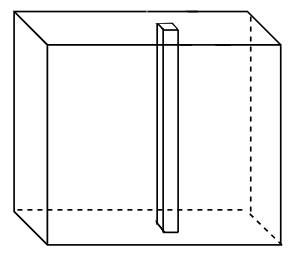
\includegraphics[height=4cm]{Images/theory/voxel.png}
  \caption{Resulting scan}
  \label{fig:voxel2}
\end{figure}


\subsection{Line Scanning Image} \label{sec:push}
The line scanning image technique uses a two-dimensional detector, perpendicular/orthogonal to the surface of the measured target. This detector collects the spectrum of a whole line in the image, in one single scan. By moving the scan line with a push broom technique, one can map the entire image by combining all sets of spectra.

% \begin{figure}[H]
% \centering
%   \includegraphics[height=12cm]{Images/theory/linescan.png}
%   \caption{Set-up, Line Scanning Image}
%   \label{fig:linescan}
% \end{figure}

\begin{figure}[H]
\centering
  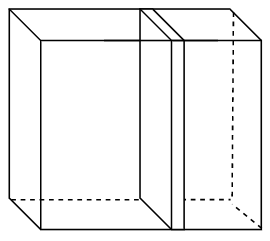
\includegraphics[height=4cm]{Images/theory/pushbroom.png}
  \caption{ Resulting scan}
  \label{fig:pushbroom}
\end{figure}

\section{SINTEF SilCam}
%https://github.com/emlynjdavies/PySilCam/wiki 
The silhouette camera, SINTEF SilCam, is a holographic imager designed to overcome the limitations in depth-of-field scenarios related to restricted path length, which is a challenge when using today's conventional lens-based imaging. The imager is developed by SINTEF with one of the experts, Emlyn Davies, in the front.
\\\\
In order to reduce noise, each image is corrected using a clean background. This is done by guiding the object into a control volume, rapidly illuminated through a diffuser causing a uniformly illuminated white surface background. From this, it is possible to produce a logical image of the particles detected, containing only zeros and ones. In turn, particle properties for each particle can be calculated from the binary image.
This way, the background enables the CCD, or simply a camera, to capture the silhouette of the particle.
\\\\
This way, the system can be used for both large- and small-scale experiments. In smaller scale, the SilCam is able to quantify the distribution of suspended material. Zoo-plankton, larger phyto-plankton, mineral grains and marine snow are all examples of objects the SilCam can detect. 



\chapter{Data Tracking and Analysis} \label{cap:theory3}
This chapter presents ways of tracking and handling data. The data collected in this thesis has been analyzed through a principal component analysis, extracting information to be viewed as relevant only and disregarding the rest. Section \ref{sec:pca}, regarding PCA theory, contain knowledge gained in TTK19...\todo{kilde}. In this thesis, the data collected is from physical samples of the five types of microplastic - also elaborated at the beginning of this chapter.

\section{Microplastic} \label{sec:microplastic}
%ha med hva def av mikroplast og de ulike plasttypene
%Kjemi
\todo[inline, color=orange!40]{ta med figur av alles struktur?}
\noindent
As mentioned, plastics have permeated almost every aspect of modern day life with its large applicability. We find plastic in the microchips in our computers, as well as in the bags we carry our groceries in. It seems that plastic covers a wide spectrum of applications.  One reason to this, is the many different types of plastic, covering different areas of need. Polyethylene (PE), polypropylene (PP), polyethylene terephthalate (PET), polyvinyl chloride (PVC) and polystyrene (PS), are the five most common types of plastic, in large part covering of the global plastic production. Besides containing Carbon-Hydrogen bindings, these are all structurally different and they are classified according to their chemical structure. In this section, these five types of plastic are presented in decreasing order. 

%Plastic polymers commonly found in the environment are polypropylene (PP), polyethylene (PE), polyethylene terephthalate (PET), polystyrene (PS) and polyvinylchloride (PVC).8 Together these comprise 72.9 percent of the plastic produced globally.9

\subsection{Polyethylene}
The monomers in polyethylene (PE) has the chemical formula $C_2H_4$. Polyethylene is the most common type of plastic. The reason to its commonness is the broad application of it in consumer products. Plastic bags, bottles and food wrapping are good examples of polyethylene. However, these three products seem to have a significantly different material. For instance are plastic bags rarely as rigid and as bottles. This variation in polyethylene creates two sub-types defined by the degree of density – HDPE and LDPE, high-density polyethylene and low-density polyethylene respectively. 
\\\\
The LPDE-monomers are more branched, meaning that a chain is replacing for instance a hydrogen atom. As a result of this, the monomers are less tightly packed, leading to a lower density.  As LDPE has more branching than HDPE, its intermolecular forces are weaker.


\subsection{Polypropylene}
Polypropylene (PP) is the second most common plastic consistent of propylene with the chemical formula $C_3H_6$. PP has properties similar to polyethylene, but it is slightly harder and more resistant to fatigue. The plastic type is found in a variety of products like food packaging, labeling and clothing. 

\subsection{Polyvinyl Chloride}
%http://www.plasticmoulding.ca/polymers/pvc.htm
Polyvinyl chloride (PVC) with a number of vinyl chloride monomers formulated by $C_2H_3Cl$, is in third place of the most produced types of plastic. PVC can be both rigid and flexible. The rigid form is used in constructional application in piping and electrical wire insulation, while the softer and more flexible form is used in many applications replacing rubber. 

\subsection{Polyethylene terephthalate}
Polyethylene terephthalate (PET) consist of repeating ethylene terephthalate monomers, holding the chemical formula $C_{10}H_8O_4$. Typically PET is used in plastic bottles and in fibers for clothing. For the latter use, the type is commonly known as polyester. Depending on the specific particle's size and crystal structure, the semi crystalline material, PET, might appear transparent. 

\subsection{Polystyrene}
%https://www.azom.com/article.aspx?ArticleID=7915
Polystyrene (PS) is an inexpensive plastic type commonly used for packaging purposes, with the chemical formula being $(C_8H_8)_n$. PS increasingly exists in the outdoor environment, particularly along shores. The plastic is naturally clear, hard and brittle. The latter fact is perhaps the main reason to why larger pieces of PS easily turn into microplastic. 

\section{Georeferencing}
%http://www.gisresources.com/georeferencing-2/
In raster system, points are represented by single cells, lines by sequence of neighboring cells and area by collection of continuous cells
\\\\
%http://desktop.arcgis.com/en/arcmap/10.3/manage-data/raster-and-images/fundamentals-for-georeferencing-a-raster-dataset.htm
Georeferencing means to relate an internal coordinate system to a spatial coordinate system. The internal coordinate system could for instance be a raster image of a map. 
%http://www.gisresources.com/georeferencing-2/
Note that raster systems represents points by single cells and lines by several neighboring cells. Areas are represented by a collection of continuous cells. 
\\\\
In order to georeference an image, control points need to be established. These control points are identified as a series of known x- and y-coordinates, linking locations in the raster dataset to its correspondant location in the spatially referenced data. The desired objective is to assign these coordinate systems to each other with minimal residuals. This means that the distance between the control points’ actual coordinates and the coordinates predicted by the model is the smallest is can be, making the process as accurate as possible. This way, georeferencing can explain how data, such as GPS points, are related to images.

\section{Principal Component Analysis} \label{sec:pca}
The main purpose of conducting a principal component analysis (PCA) is to extract only relevant and therby useful information from the dataset. The analysis converts a set of observations of possibly correlated variables into a set of values of linearly uncorrelated variables called principal components. These principal components will describe the overall variation of the dataset and thereby serve as a latent variable. In most cases, only two or three principal components explain almost the entire dataset. By disregarding the remaining percentage (which often is explained with several components), the dimension of the dataset is reduced. In most cases, this reduction reveals and highlights only the relevant variations. In addition, a reduced set will often have a decreased error rate because of the lower amount of variables connected to the sample, excluding the relations typically regarded as noise. Lastly, the resulting set will have a lower computational time and thereby cost.
\\\\
Now, how are these principal components found? Figure \ref{fig:pca1} a) describes the entire dataset with one dot describing one sample/single data observation. The analysis begins with finding the projection of each observation onto a line. The line is drawn with the purpose of explaining as many observations as possible, but minimizing the total distance between the samples and their projection. This resulting line is illustrated in \ref{fig:pca1}b). The distance from the origin to this projected point along the line is the score associated with the related observation. 
%The direction of the line is now characterized with giving the largest variance of the scores, and is described by direction vectors called loadings. 
\\\\
%Simply put, the original data is estimated by multiplying the scores with the associated loadings.
\noindent
This way, the first line created as the highest variance. This line is called the first principal component. When creating an additional space, the new component needs to be uncorrelated with the others. The second principal component, illustrated in \ref{fig:pca1}c), is therefore perpendicular to the first component’s direction, but is otherwise found the same way. This way, the first principal component has the largest possible variance. Each following component will, in turn, have the highest variance possible under the constraint that it is perpendicular to the previous components.
\\\\
Of the results it is often possible to detect trends and clusters. This is typically for unsupervised learning, where the purpose is to gain knowledge about the samples relative to each other. This way, one can learn what factors provide the variation of the data and how the samples are correlated – even if the preknowledge regarding the dataset is next to nothing. 
%FIGURENE:
%https://learnche.org/pid/latent-variable-modelling/principal-component-analysis/geometric-explanation-of-pca
\begin{figure}[H]
  \newcommand*\FigVSkip{0.5em}
  \newcommand*\FigHSkip{0.1em}
  \newsavebox\FigBox
  \centering
  % Top image is centered, so no need to get width
\sbox{\FigBox}{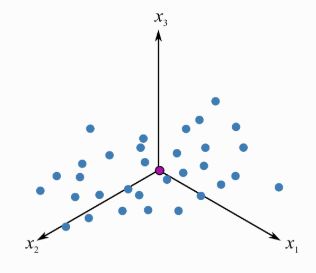
\includegraphics[scale=0.4]{Images/theory/koord.png}}
  \begin{minipage}{\wd\FigBox}
    \centering\usebox{\FigBox}
    \subcaption{a) Scaled and centered data observations}
  \end{minipage}
 \sbox{\FigBox}{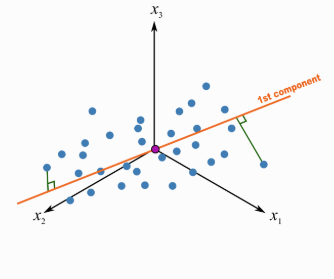
\includegraphics[scale=0.4]{Images/theory/1pc.png}}
  \begin{minipage}{\wd\FigBox}
    \centering\usebox{\FigBox}
    \subcaption{\newline b) Including first principal component}
  \end{minipage}
  % Save first image in a box to get the width
  \sbox{\FigBox}{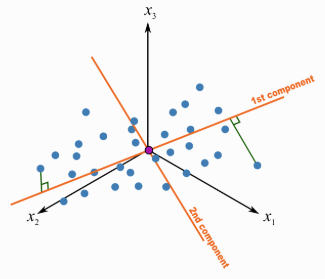
\includegraphics[scale=0.4]{Images/theory/2pc.png}}
  \begin{minipage}{\wd\FigBox}
    \centering\usebox{\FigBox}
    \subcaption{c) Including second principal component}
  \end{minipage}\hspace*{\FigHSkip}
  % Save second image 
  \caption{Coordinate system with observations and principal components}
  \label{fig:pca1}
\end{figure}


%https://learnche.org/pid/latent-variable-modelling/principal-component-analysis/interpreting-the-residuals
\subsection{Scores}
As mentioned, every sample has an associated score described by the distance along the principal component from the origin to the projected point of the sample. All scores of the reduced dataset are represented in a scatter plot. As the axes in this plot are fully consistent of the used principal components, it is possible to interpret the original data by detecting patterns in the score plot. 
\\\\
Now, how are these pattern detected? When searching for patterns it is common to look for clustering of samples indicating correlation between the samples due to similar values at a high degree of the variables. This will, in turn, indicate similar properties for the clustered samples. In addition, outliers can be found as a lonely sample located away from the rest of the set. Outliers are important as they may affect the result even more than the rest of the set, pulling the result in the direction of its location. Either the deviation is explainable, indicating that the sample should remain, or the sampling process has been noisy, making the outlier non-representable. In the latter case, the sample should be removed from the set. 

\subsection{Loadings}
The amount of influence each variable has on the principal components, defines the associated loading. This can be interpreted from the loadings plot, as its axes determines the effect the variables has on the first and second component, respectively (or any other component included in the reduced set). This way, a low loading is dedicated to variables with low contribution and vice versa. 

\subsection{Residuals}
Residuals describe the deviation in the predicted values. The residual plot is therefore a good visual indication of how well aligned the model is in reference to the actual measurements. The plot contains lines separating the samples at a given deviation percentage. This way, samples with residuals above this line, can for instance be interpreted further.
\\\\
Whenever large deviations occur, a contribution plot can be analyzed. A contribution plot is a visualization of the residuals for each principal component, making it easier to determine the cause of the deviation. 

\subsection{Hotelling's $T^2$} \label{sec:hotellings}
Hotellings $T^2$ is simply the summation of all scores. Nevertheless, these results are very useful, especially when detecting outliers. The resulting plot consists of two ellipses defining two intervals in percent. The percentage determining these intervals value, but they are normally based on the confidence interval in a normal distribution - typically 95\% for the inner ellipse and 99\% for the outer. Normally the variables of the inner circle turns out to be more significant than the outer. 

\subsection{Hotelling's $T^2$ VS Residual} \label{sec:vs}
The plot consistent of the hotelling’s $T^2$ values on the x-axis and residuals on the y-axis, is called a influence or leverage plot. This plot can be divided into four sections describing the relation between leverage and deviation of an observation. Bottom left contains low leveraged data with small deviations, while top right describes data with high influence and high associated residuals. It is especially important to detect an analyze the observations with both large deviation and large leverage, as these affect the results to a high degree while at the same time possibly pulling the results in the wrong direction (due to error). 


